\documentclass[10pt,a4paper]{report}
\usepackage[utf8]{inputenc}
\usepackage{amsmath}
\usepackage{amsfonts}
\usepackage{amssymb}
\usepackage{graphicx}
\usepackage{color}

\topskip0pt
\setlength{\parskip}{0em}
\begin{document}

\pagebreak
\vspace*{\fill}
\begin{center}
\begin{LARGE}
Network Configuration

\end{LARGE}
\begin{Large}
Rwithik Manoj\\
20-02-2019
\end{Large}
\end{center}
\vspace*{\fill}
\pagebreak

\begin{center}
\begin{Large}
About ifconfig
\end{Large}
\end{center}

\begin{flushleft}
ifconfig, short for ``interface configuration" is used to configure, manage and query network interface parameters via command line interface or in system configuration scripts for system/network management in Unix/Linux operating systems. \par
The command ``ifconfig" is used to display current network configuration information, set up an ip address, netmask or broadcast address on a network interface, create an alias for a network interface, set up a hardware address and enable or disable network interfaces.\\
\medskip
Using {\color{red} ifconfig} with no parameters display the information about the network interfaces that are currently up.\\
\medskip
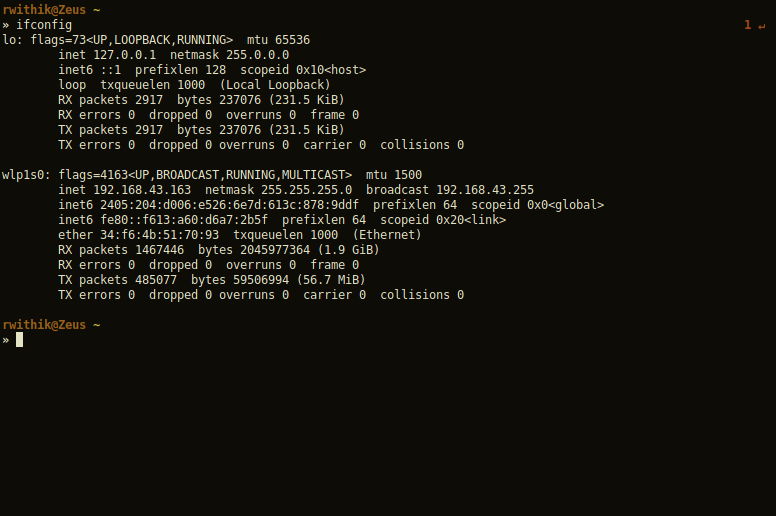
\includegraphics[scale=.5]{../Images/Network/1.png}

\pagebreak
Using the -a flag displays all the interfaces, even the ones which are down.\\
\medskip
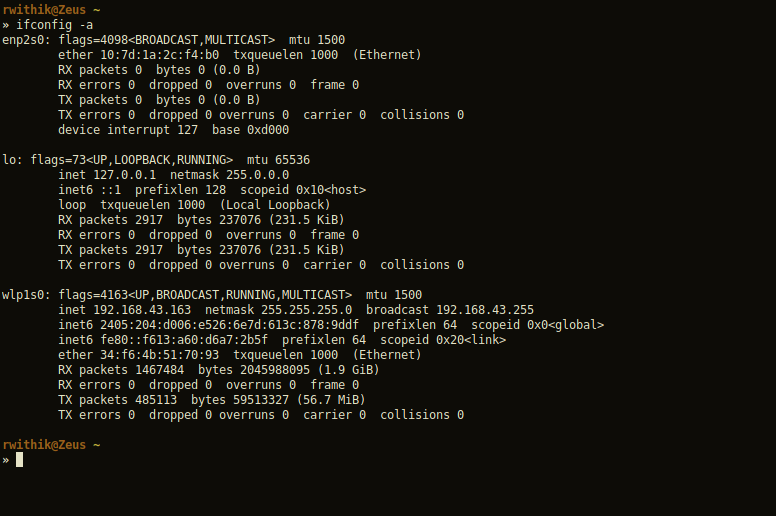
\includegraphics[scale=.5]{../Images/Network/2.png}\\
\medskip
Using {\color {red} ifconfig [INTERFACE NAME]} will display the information about the mentioned interface.\\\medskip
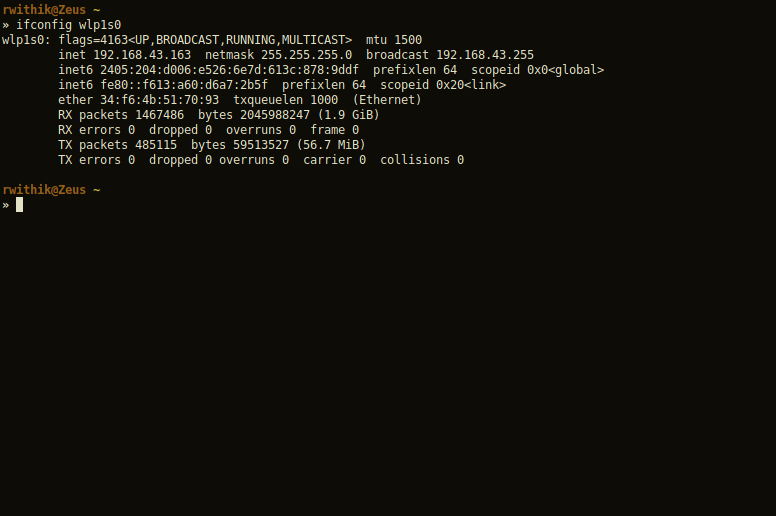
\includegraphics[scale=.5]{../Images/Network/3.png}

\pagebreak
Disabling and enabling interfaces with ifconfig.\\
Syntax: {\color{red} ifconfig [INTERFACE] [up/down]}\\\medskip
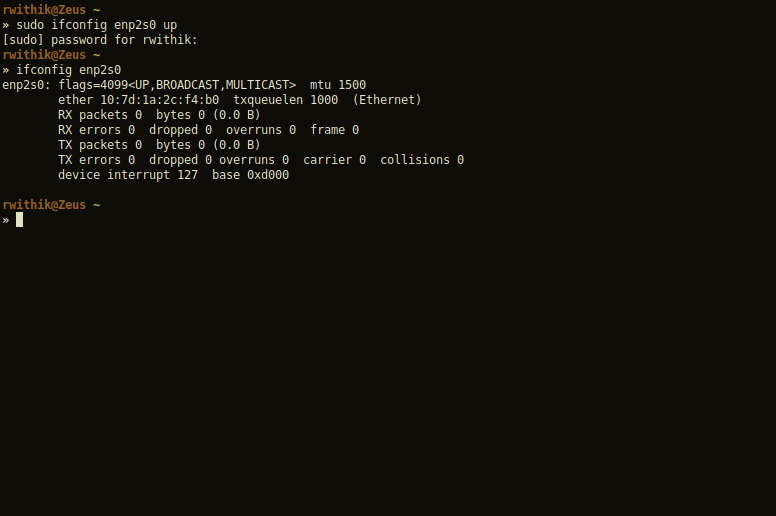
\includegraphics[scale=.5]{../Images/Network/4.png}\\\medskip

\pagebreak
\vspace*{\fill}
\begin{center}
\begin{large}
What is a gateway?
\end{large}
\end{center}

A gateway is a network node that connects two networks using different protocols together. The most common gateway is the router. It connect home networks to the internet.
\par The gateway can be set using the {\color{red} ip route} or {\color{red} ip r} command.\\

Syntax: ip route add default via [GATEWAY] dev [INTERFACE]\\

Example: ip route add default via 192.168.0.254 dev eth0, assuming 192.168.0.254 is the ip of your gateway.
\vspace*{\fill}
\pagebreak
\vspace*{\fill}
\begin{center}
\begin{large}
What is a DNS
\end{large}
\end{center}

DNS, or Domain Name Server, translates the domain names to IP addresses, so that the browser can interact with them. Each device connected to the Internet has a unique IP address which other machines use to find the device. DNS servers allows us to simply type the domain as example.com, and be taken to the website instead of typing the IP address of the domain.\\
\medskip
Your DNS information is stored in {\color{blue} \textbackslash{}etc\textbackslash{}resolve.conf}\\
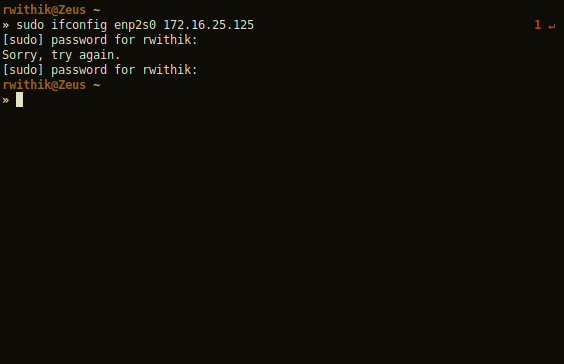
\includegraphics[scale=.5]{../Images/Network/5.png}\\ 
\medskip 
Just edit this file to set a custom DNS.
\vspace*{\fill}
\pagebreak
\vspace*{\fill}
\begin{center}
\begin{Large}
About iptables
\end{Large}
\end{center}

Iptables is a firewall tool include in the Linux netfilter framework. A firewall is a network security system that monitors and controls on the basis of predetermined security rules incoming and outgoing network traffic.
Use {\color{red} iptables -L} to list the current rules.\\
\medskip
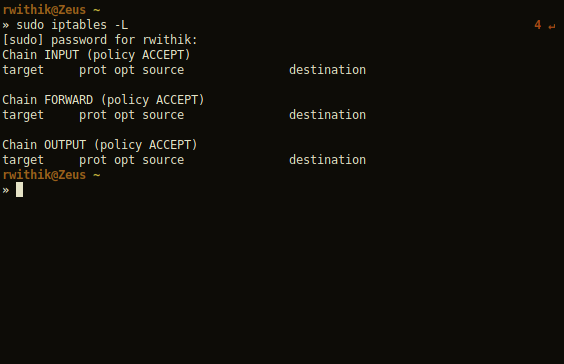
\includegraphics[scale=.5]{../Images/Network/6.png}\\
\medskip
There are two policies- ACCEPT and DENY. 
ACCEPT allows packages to be received from the mentioned IP addresses. And DROP blocks them.

For Example, if the default policy of INPUT is DROP, iptables blocks all incoming packages.\\
To allow all packages from your LAN, run this command to add rule to your iptables.\\
iptables -A INPUT -s 192.168.100.0/24 -j ACCEPT\\


\end{flushleft}
\vspace*{\fill}
\pagebreak

\end{document}